\documentclass{standalone}
\usepackage{tikz}  %TikZ central library is called.
\usetikzlibrary{automata,positioning} 
\tikzset{%
  every neuron/.style={
    circle,
    draw,
    minimum size=0.8cm
  },
  neuron missing/.style={
    draw=none, 
    scale=2,
    text height=0.2cm,
    execute at begin node=\color{black}$\vdots$
  }
 }

\begin{document}
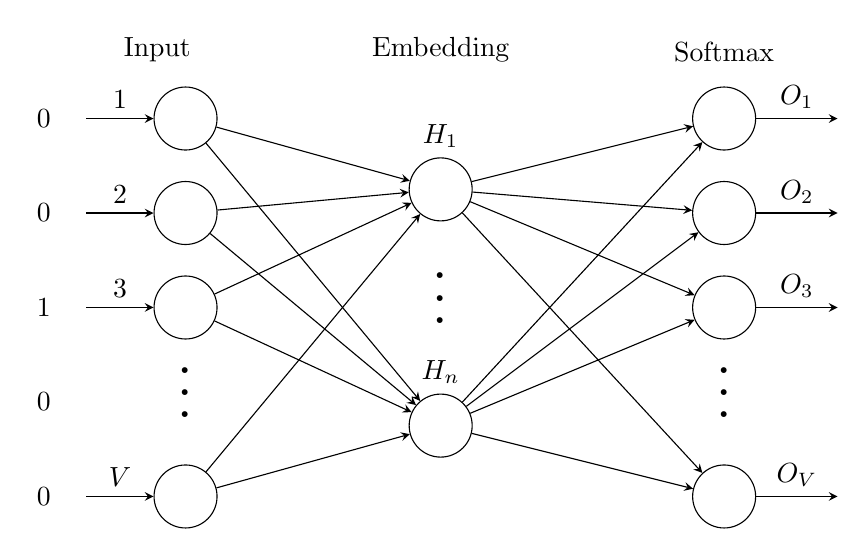
\begin{tikzpicture}[x=1.8cm, y=1.2cm, >=stealth]

\foreach \m/\l [count=\y] in {0, 0 , 1, 0 ,0}
  \node [every neinput/.try, neinput \m/.try] (input-\m) at (-0.8, 2.5-\y) {$\m$};
  
\foreach \m/\l [count=\y] in {1,2,3,missing,4}
  \node [every neuron/.try, neuron \m/.try] (input-\m) at (0.2,2.5-\y) {};

\foreach \m [count=\y] in {1,missing,2}
  \node [every neuron/.try, neuron \m/.try ] (hidden-\m) at (2,2-\y*1.25) {};

\foreach \m [count=\y] in {1,2, 3, missing,4}
  \node [every neuron/.try, neuron \m/.try ] (output-\m) at (4,2.5-\y) {};

\foreach \l [count=\i] in {1,2,3,V}
  \draw [<-] (input-\i) -- ++(-0.7,0)
    node [above, midway] {$\l$};

\foreach \l [count=\i] in {1, n}
  \node [above] at (hidden-\i.north) {$H_\l$};

\foreach \l [count=\i] in {1,2, 3, V}
  \draw [->] (output-\i) -- ++(0.8,0)
    node [above, midway] {$O_\l$};

\foreach \i in {1,...,4}
  \foreach \j in {1,...,2}
    \draw [->] (input-\i) -- (hidden-\j);

\foreach \i in {1,...,2}
  \foreach \j in {1,...,4}
    \draw [->] (hidden-\i) --(output-\j);

\foreach \l [count=\x from 0] in {Input, Embedding, Softmax}
  \node [align=center, above] at (\x*2,2) {\l };

\end{tikzpicture}
\end{document}